% vim: set textwidth=78 autoindent:

\section{Lavorare con i dati raster}\label{label_raster}
\index{raster layers|(}

% when the revision of a section has been finalized, 
% comment out the following line:
%\updatedisclaimer

Questa Sezione descrive come visualizzare ed impostare le proprietà dei dati
raster. I formati raster attualmente supportati in QGIS includono:\index{raster layers!data formats}

\begin{itemize}
\item Arc/Info Binary Grid
\item Arc/Info ASCII Grid
\item GRASS Raster
\item GeoTIFF
\item JPEG
\item Spatial Data Transfer Standard Grids (con alcune limitazioni)
\item USGS ASCII DEM
\item Erdas Imagine
\end{itemize}

Considerato che il supporto ai raster in QGIS è fornito dalla libreria GDAL,
oltre a quelli elencati è possibile che sia possibile caricare anche altri
formati supportati da GDAL - nel dubbio è comunuque possibile provare ad aprire il file
in QGIS per verificare l'esito. Ulteriori dettagli sono forniti all'Appendice \ref{appdx_gdal}
\index{raster layers!GDAL implementation} o all'indirizzo
\url{http://www.gdal.org/formats_list.html}. Per caricare dati raster di
GRASS, fare riferimento alla Sezione~\ref{sec:load_grassdata}.

\subsection{Cosa sono i dati raster?}\label{label_whatsraster}
\index{raster layers!definition}

I dati raster nei GIS sono matrici di celle discrete che rappresentano le
caratteristiche della superficie terrestre o dell'ambiente al di sopra o al di sotto
di essa. Ogni cella nella matrice raster presenta lo stesso formato e le celle
sono solitamente rettangolari (in QGIS saranno sempre rettangolari). Esempi
tipici di dati raster sono quelli provenienti dal telerilevamento come le
fotografie aeree o immagini proveniente dal satellite e dati
modellistici quali matrici dell’altitudine.

Diversamente dai dati vettoriali, i dati raster di solito non hanno associato
un database contenente i dati descrittivi di ogni cella.

I dati raster, infine, sono geocodificati in base alla risoluzione del pixel e
alle coordinate x/y di un angolo del raster che ne consente un corretto
posizionamento nella vista mappa. 

QGIS utilizza le informazioni di georeferenziazione incorporate nel layer
raster (ad es. GeoTiff) o in un apposito "world file" per visualizzare
correttamente i dati.\index{raster layers!georeferenced}
	
\subsection{Caricati dati raster in QGIS}\label{label_loadraster}

I layer raster possono essere caricati sia selezionando nella barra lo
strumento \toolbtntwo{mActionAddRasterLayer}{Aggiungi layer raster} o
scegliendo la voce di menù
\mainmenuopt{Layer}>\dropmenuopttwo{mActionAddRasterLayer}{Aggiungi layer
raster}. È possibile caricare più di un livello alla volta tenendo premuto il
tasto \keystroke{Control} o \keystroke{Shift} mentre si effettua la selezione
multipla con il mouse sui livelli nella finestra di dialogo \dialog{Apre
unraster supportato da GDAL}.\index{raster layers!loading}

Quando il layer è caricato è possibile cliccare nella legenda sul relativo
nome con il tasto destro per selezionare ed attivare opzioni specifiche o per
aprire la finestra per l'impostazione delle proprietà del layer raster.

\minisec{Menù contestuale per layers raster}

\begin{itemize}
\item \dropmenuopt{Zoom all'estensione del layer}
\item \dropmenuopt{Zoom alla scala migliore (100\%)}
\item \dropmenuopt{Aggiungi alla panoramica}
\item \dropmenuopt{Rimuovi}
\item \dropmenuopt{Proprietà}
\item \dropmenuopt{Rinomina}
\item \dropmenuopt{Aggiungi gruppo}
\item \dropmenuopt{Espandi tutto}
\item \dropmenuopt{Comprimi tutto}
\item \dropmenuopt{Mostra gruppi}
\end{itemize}
	
\subsection{Finestra delle proprietà raster}\label{label_rasterprop}

Per visualizzare ed impostare le proprietà di un layer raster, fare doppio
click sul nome del raster nella legenda o cliccare su di esso con il tasto
destro e scegliere \dropmenuopt{Proprietà} dal menù contestuale:\index{raster layers!context menu}
La figura \ref{fig:raster_properties} mostra la finestra \dialog{Proprietà raster}. 
Ci sono diverse linguette nella finestra: 

\begin{itemize}
 \item \tab{Simbologia}
 \item \tab{Trasparenza}
 \item \tab{Mappa colore}
 \item \tab{Generale}
 \item \tab{Metadata}
 \item \tab{Piramidi}
 \item \tab{Istogramma}
\end{itemize}

\begin{figure}[h]
  \begin{center}
   \caption{Finestra delle proprietà dei livelli raster \nixcaption}\label{fig:raster_properties}\smallskip
   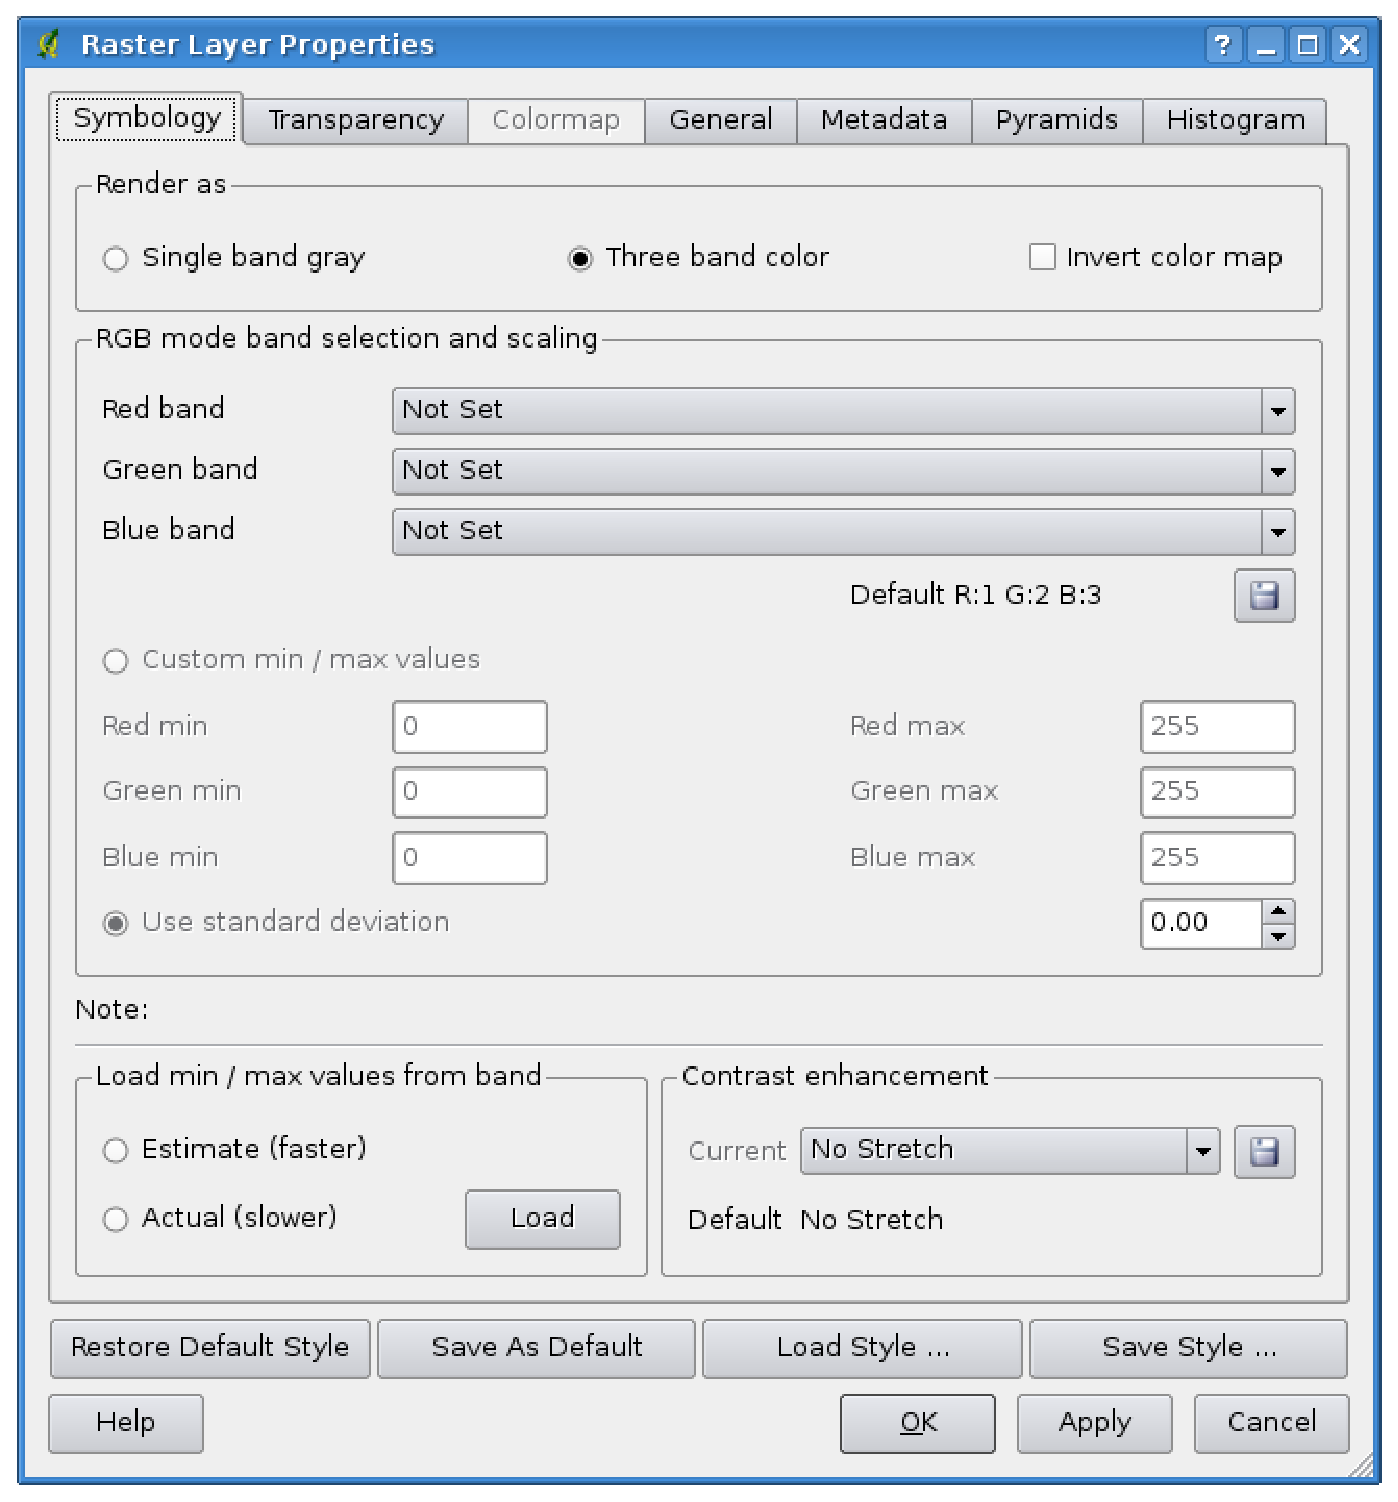
\includegraphics[clip=true, width=14cm]{rasterPropertiesDialog}
\end{center}  
\end{figure}

\subsubsection{Linguetta Simbologia}\label{label_sombology}

QGIS può rendere a video i raster in due modi:\index{raster layers!supported channels}

\begin{itemize}
\item Banda singola grigia - viene campionata una sola banda dell'immagine e
resa in gradazioni di grigio o in pseudocolore.
\item Tre bande di colore - vengono rese a video tre bande dell'immagine
ognuna rappresentante le componenti rosso, verde o blu che saranno composte
per creare un'immagine a colori.
\end{itemize}

È possibile invertire i colori in modo che i colori chiari divengano scuri e
viceversa selezionando la casella di controllo \checkbox{Inverti mappa colore}.

\minisec{Resa in banda singola}

Selezionando questa opzione vengono offerte due possibilità tra le quali
scegliere. Innanzitutto se il layer è multibanda è possibile scegliere quale
banda si desidera venga impiegata per la resa a video. 

La seconda opzione offre una selezione di tabelle colori preimpostate per la
resa a video.

Le scelte possibili disponibili nel menù a tendina sono
\selectstring{Mappa colore}{Scala di grigi}, impostazione di default.
Altre scelte possibili sono
\begin{itemize}
\item Pseudo colore
\item Freak Out
\item Mappa colore
\end{itemize}

Quando viene selezionata l'opzione \selectstring{Mappa colore}{Mappa colore},
viene abilitata la linguetta \tab{Mappa colore}. Si vedano ulteriori
informazioni al capitolo \ref{label_colormaptab}.

Per immagini in pseudocolore in QGIS è possibile limitare i dati visualizzati
per mostrare soltanto le celle i cui valori ricadono all'interno di una deviazione standard
definita.\index{raster layers!standard deviation} Ciò può essere utile quando
nella griglia raster si hanno una o due celle con valori anormalmente alti
che hanno un impatto negativo sulla resa a video del raster.

\minisec{Resa in tre bande}

This selection offers you a wide range of options to modify the appereance
of your rasterlayer. For example you could switch color-bands from the
standard RGB-order to something else.

Also scaling of colors are available.


\begin{Tip}\caption{\textsc{Viewing a Single Band of a Multiband Raster}}
\qgistip{If you want to view a single band (for example Red) of a multiband
image, you might think you would set the Green and Blue bands to ``Not
Set''. But this is not the correct way. To display the Red band, 
set the image type to grayscale, then select Red as the band to use for Gray.
}
\end{Tip} 

\subsubsection{Transparency Tab} \label{rastertab:transparency}

QGIS has the ability to display each raster layer at varying transparency
levels.\index{raster layers!transparency} Use the transparency slider to indicate to
what extent the underlying layers (if any) should be visible though the
current raster layer. 
This is very useful, if
you like to overlay more than one rasterlayer, e.g. a shaded relief-map
overlayed by a classified rastermap. This will make the look of the map
more three dimensional.

Additionally you can enter a rastervalue, which should be treated as
{\em NODATA}.

An even more flexible way to customize the transparency can be done in the
\guiheading{Custom transparency options} section.
The transparency of every pixel can be set in this tab.

As an example we want to set the water of our example rasterfile
\filename{landcover.tif} to a transparency of 20\%. The following steps
are neccessary:
\begin{enumerate}
 \item  Load the rasterfile \filename{landcover}
 \item Open the \dialog{properties} dialog by double-clicking on the
 rasterfile-name in the legend or by right-clicking and choosing
 \dropmenuopt{Properties} from the popup meun.
 \item select the \tab{Trasparenza} tab
 \item \label{enum:add} Click the \toolbtntwo{mActionNewAttribute}{Add values manually}
 button. A new row will appear in the pixel-list.
 \item \label{enum:transp} enter the the raster-value (we use 0 here) and adjust the
 transparency to 20\%
 \item press the \button{Apply} button and have a look at the map
\end{enumerate}

You can repeat the steps \ref{enum:add} and \ref{enum:transp} to adjust
more values with custom transparency.

As you can see this is quite easy set custom transparency, but it can be
quite a lot of work. Therefor you can use the button
\toolbtntwo{mActionFileSave}{Export to file} to save your
transparency-list to a file. The button
\toolbtntwo{mActionAddRasterLayer}{Import from file} loads your
transparency-settings and applies them to the current rasterlayer.

\subsubsection{Mappa colore} \label{label_colormaptab}
% FIXME: Write me

The \tab{Mappa colore} tab is only available, when you have selected a
single-band-rendering within the tab \tab{Simbologia} (see chapt. \ref{label_sombology}).

Three ways of color interpolation are available:
\begin{itemize}
\item Discrete
\item Linear 
\item Exact
\end{itemize}

The button \button{Add Entry} adds a color to the individual color-table.
Double-Clicking on the value-column lets you inserting a specific value.
Double clicking on the color-column opens the dialog \dialog{Select
color} where you can select a color to apply on that value.

Alternativly you can click on the button
\toolbtntwo{mActionNewAttribute}{Load colormap from Band}
, which tries to
load the table from the band (if it has any).

The block \guiheading{Generate new color map} allows you to create newly
categorized colormaps. You only need to select the \selectnumber{number of
classes}{15} you need and press the button \button{Classify}. Currently
only one \selectstring{Classification mode}{Equal Interval} is
supported\index{raster layer!classify}.

\subsubsection{General Tab}\label{label_generaltab}

The \tab{Generale} tab displays basic information about the selected raster,
including the layer source and  display name in the legend (which can be
modified). This tab also shows a thumbnail of the layer, its legend symbol,
and the palette.\index{raster layers!properties}

Additionally scale-dependent visability can be set in this tab. You need to
check the checkbox and set an appropriate scale where your data will be
displayed in the map canvas.

Also the spatial reference system is printed here as a PROJ.4-string. 
This can be modified by hitting the \button{Change} button.

\subsubsection{Metadata Tab}\label{label_metatab}

The \tab{Metadata} tab displays a wealth of information about the raster layer,
including statistics about each band in the current raster layer. Statistics
are gathered on a 'need to know' basis, so it may well be that a given layers
statistics have not yet been collected.\index{raster layers!metadata}

This tab is mainly for information. You cannot change any values printed
inside this tab. To update the statistics you need to change to tab
\tab{Istogramma} and press the button \button{Refresh} on the bottom right,
see ch. \ref{label_histogram}.

\subsubsection{Pyramids Tab}\label{raster_pyramids}

Large resolution raster layers can slow navigation in QGIS. By creating lower
resolution copies of the data (pyramids), performance can be considerably
improved as QGIS selects the most suitable resolution to use depending on the
level of zoom.
\index{raster layers!pyramids}
\index{raster layers!resolution pyramids}

You must have write access in the directory where the original data is stored
to build pyramids. \\
Several resampling methods can be used to calculate the pyramides:
\begin{itemize}
\item Average
\item Nearest Neighbour
\end{itemize}

When checking the checkbox \checkbox{Build pyramids internally if
possible} QGIS tries to build pyramids internally.

Please note that building pyramids may alter the original data file and once
created they cannot be removed. If you wish to preserve a 'non-pyramided'
version of your raster, make a backup copy prior to building pyramids.

\subsubsection{Histogram Tab}\label{label_histogram}

The \tab{Istogramma} tab allows you to view the distribution\index{raster layers!histogram} 
of the bands or colors in your raster. You must first generate the raster statistics 
by clicking the \button{Refresh} button. You can choose which bands to display by 
selecting them in the list box at the bottom left of the tab. Two different
chart types are allowed: 

\begin{itemize}
\item Bar chart
\item Line graph
\end{itemize}

You can define the number of chart columns to use and decide wether you want 
to \checkbox{Allow approximation} or display \checkbox{out of range} values 
Once you view the histogram, you'll notice that the band statistics have been
populated on the \tab{metadata} tab.\index{raster layers!metadata)}

\begin{Tip}\caption{\textsc{Gathering Raster Statistics}}
\qgistip{To gather statistics for a layer, select pseudocolor rendering and
click the \button{Apply} button. Gathering statistics for a layer can be time
consuming. Please be patient while QGIS examines your
data!\index{raster layers!statistics}
}
\end{Tip}

